
% This describes the catalog services design for DODS.
% 
% $Id$

\documentclass[12pt]{article} 
\usepackage{html,epsfig,code}

%
% These are html links which are used often enough in writing about DODS to
% merit an input file.
% jhrg. 4/17/94
%
% File rationalized and updated while writing the DODS User
% Guide. Also includes other useful abbreviations.
% tomfool 3/15/96
%
% $Id$
%
% HTML references to DODS documents
%
% For most of the DODS documentation there are three html references defined:
% 1) The upper case \newcommand produces the title of the paper, an
%    html link in the online documentation and a footnote in the paper
%    version.  
% 2) A capitalized version produces a capitalized description of the
%    paper and a link in the online version (but no footnote in the
%    paper version). 
% 3) A lower case version which produces a lower case description of
%    the paper and a html link, but no footnote.

% External references to documents:
%
% In order for external references to work (via latex2html) the labels used
% throughout the documents must be unique. The text labels are all prefixed
% with a document identifier (e.g., ddd) with a colon separater. The
% \externalrefs below (way below...) includes the perl files html.sty uses to
% make the cross refs.

\newcommand{\DODS}{\htmladdnormallink{Distributed Oceanographic Data System}
  {http://www.unidata.ucar.edu/packages/dods/}}

\newcommand{\Dods}{\htmladdnormallink{DODS}{http://www.unidata.ucar.edu/packages/dods/}}

\newcommand{\wrkshp}{\htmladdnormallink{Report on the First Workshop for the
    Distributed Oceanographic Data System, Proposed System Architectures}
  {http://www.unidata.ucar.edu/packages/dods/archive/reports/workshop1/section3.13.html}}

% not DODS URLs, but useful all the same...

\newcommand{\www}{\htmladdnormallink{World Wide Web} 
  {http://www.w3.org/hypertext/WWW/TheProject.html}}
\newcommand{\url}{\htmladdnormallink{Uniform Resource Locator}
  {http://www.w3.org/hypertext/WWW/Addressing/URL/url-spec.html}}

\newcommand{\uri}{\htmladdnormallinkfoot{Uniform Resource Identifiers}
  {http://www.w3.org/hypertext/WWW/Addressing/URL/uri-spec.html}}

\newcommand{\urn}{\htmladdnormallinkfoot{Uniform Resource Name}
  {http://www.acl.lanl.gov/URI/archive/uri-archive.messages/1143.html}}

\newcommand{\HTTPD}{\htmladdnormallinkfoot{HTTPD}
  {http://hoohoo.ncsa.uiuc.edu/docs/Overview.html}}

\newcommand{\HTTP}{\htmladdnormallinkfoot{HyperText Transfer Protocol}
  {http://www.w3.org/hypertext/WWW/Protocols/HTTP/HTTP2.html}}

%\newcommand{\HTML}{\htmladdnormallinkfoot{HyperText Markup Language}
%  {http://www.w3.org/hypertext/WWW/MarkUp/MarkUp.html}}

% CERN used to be `Conseil Europeen pour la Recherche Nucleaire'
\newcommand{\CERN}
  {\htmladdnormallink{European Laboratory for Particle Physics}
  {http://www.cern.ch/}}

\newcommand{\NCSA}
  {\htmladdnormallink{National Center for Supercomputing Applications}
  {http://www.ncsa.uiuc.edu/}}

\newcommand{\WWWC}{\htmladdnormallink{World Widw Web Consortium}
  {http://www.w3.org/}}

\newcommand{\CGI}{\htmladdnormallinkfoot{Common Gateway Interface}
  {http://hoohoo.ncsa.uiuc.edu/cgi/overview.html}}

\newcommand{\MIME}{\htmladdnormallink{Multipurpose Internet Mail Extensions}
  {http://www.cis.ohio-state.edu/htbin/rfc/rfc1590.html}}

\newcommand{\netcdf}{\htmladdnormallink{NetCDF}
  {http://www.unidata.ucar.edu/packages/netcdf/guide.txn_toc.html}}

\newcommand{\JGOFS}{\htmladdnormallink{Joint Geophysical Ocean Flux Study}
  {http://www1.whoi.edu/jgofs.html}}

\newcommand{\jgofs}{\htmladdnormallink{JGOFS}
  {http://www1.whoi.edu/jgofs.html}}

\newcommand{\hdf}{\htmladdnormallink{HDF}
  {http://www.ncsa.uiuc.edu/SDG/Software/HDF/HDFIntro.html}}

\newcommand{\Cpp}{{\rm {\small C}\raise.5ex\hbox{\footnotesize ++}}}

% Commands

\newcommand{\pslink}[1]{\small
\begin{quote}
  A \htmladdnormallink{postscript}{#1} version of this document is
  available.  You may also use \htmladdnormallink{anonymous
  ftp}{ftp://ftp.unidata.ucar.edu/pub/dods/ps-docs/} to access postscript files
  of all of the DODS documentation.
\end{quote}
\normalsize
}

\newcommand{\declaration}[1]{\small
{\tt {#1}}
\normalsize
}

% All the links from here down are for the white papers. I'm not sure that any
% of these are still valid given the reorganization of the web site. 5/12/98
% jhrg.

\newcommand{\DDA}{\htmladdnormallinkfoot{DODS---Data Delivery Architecture}
  {http://www.unidata.ucar.edu/packages/dods/archive/design/data-delivery-arch/data-delivery-arch.html}}
\newcommand{\Dda}{\htmladdnormallink{Data Delivery Architecture}
  {http://www.unidata.ucar.edu/packages/dods/archive/design/data-delivery-arch/data-delivery-arch.html}}
\newcommand{\dda}{\htmladdnormallink{data delivery architecture}
  {http://www.unidata.ucar.edu/packages/dods/archive/design/data-delivery-arch/data-delivery-arch.html}}

\newcommand{\DDD}{\htmladdnormallinkfoot{DODS---Data Delivery Design}
  {http://www.unidata.ucar.edu/packages/dods/archive/design/data-delivery-design/data-delivery-design.html}}
\newcommand{\Ddd}{\htmladdnormallink{Data Delivery Design}
  {http://www.unidata.ucar.edu/packages/dods/archive/design/data-delivery-design/data-delivery-design.html}}
\newcommand{\ddd}{\htmladdnormallink{data delivery design}
  {http://www.unidata.ucar.edu/packages/dods/archive/design/data-delivery-design/data-delivery-design.html}}

\newcommand{\URL}{\htmladdnormallinkfoot{DODS---Uniform Resource Locator}
  {http://www.unidata.ucar.edu/packages/dods/archive/design/urls/urls.html}}
\newcommand{\Url}{\htmladdnormallink{Uniform Resource Locator}
  {http://www.unidata.ucar.edu/packages/dods/archive/design/urls/urls.html}}
\newcommand{\dodsurl}{\htmladdnormallink{uniform resource locator}
  {http://www.unidata.ucar.edu/packages/dods/archive/design/urls/urls.html}}

\newcommand{\DAP}{\htmladdnormallinkfoot{DODS---Data Access Protocol}
  {http://www.unidata.ucar.edu/packages/dods/archive/design/api/api.html}}
\newcommand{\Dap}{\htmladdnormallink{Data Access Protocol}
  {http://www.unidata.ucar.edu/packages/dods/archive/design/api/api.html}}
\newcommand{\dap}{\htmladdnormallink{data access protocol}
  {http://www.unidata.ucar.edu/packages/dods/archive/design/api/api.html}}

\newcommand{\SOFT}
        {\htmladdnormallinkfoot{DODS---Software Development Environment}
  {http://www.unidata.ucar.edu/packages/dods/archive/managment/software/software.html}}
\newcommand{\Soft}{\htmladdnormallink{Software Development Environment}
  {http://www.unidata.ucar.edu/packages/dods/archive/managment/software/software.html}}
\newcommand{\soft}{\htmladdnormallinkfoot{software development environment}
  {http://www.unidata.ucar.edu/packages/dods/archive/managment/software/software.html}}

% I used to call the DAP the API, then for a few days I called it the
% DTP. These def's were used then. Rather than find everywhere they are used
% (not that hard, but...) I just hacked the macros. NB: the source file for
% the DAP document is still called `api.tex'

\newcommand{\API}{\htmladdnormallinkfoot{DODS---Data Access Protocol}
  {http://www.unidata.ucar.edu/packages/dods/archive/design/api/api.html}}
\newcommand{\api}{\htmladdnormallink{data access protocol}
  {http://www.unidata.ucar.edu/packages/dods/archive/design/api/api.html}}

\newcommand{\DTP}{\htmladdnormallinkfoot{DODS---Data Access Protocol}
  {http://www.unidata.ucar.edu/packages/dods/archive/design/api/api.html}}
\newcommand{\dtp}{\htmladdnormallink{data access protocol}
  {http://www.unidata.ucar.edu/packages/dods/archive/design/api/api.html}}

\newcommand{\TOOLKIT}{\htmladdnormallinkfoot{DODS---Client and Server Toolkit}
  {http://www.unidata.ucar.edu/packages/dods/archive/implementation/toolkits/toolkits.html}}
\newcommand{\Toolkit}{\htmladdnormallink{Client and Server Toolkit}
  {http://www.unidata.ucar.edu/packages/dods/archive/implementation/toolkits/toolkits.html}}
\newcommand{\toolkit}{\htmladdnormallink{client and server toolkit}
  {http://www.unidata.ucar.edu/packages/dods/archive/implementation/toolkits/toolkits.html}}

\newcommand{\TKR}{\htmladdnormallinkfoot{DODS---DAP Toolkit Reference}
  {http://www.unidata.ucar.edu/packages/dods/archive/implementation/toolkits/toolkits.html}}
\newcommand{\Tkr}{\htmladdnormallink{DAP Toolkit Reference}
  {http://www.unidata.ucar.edu/packages/dods/archive/implementation/toolkits/toolkits.html}}
\newcommand{\tkr}{\htmladdnormallink{DAP toolkit reference}
  {http://www.unidata.ucar.edu/packages/dods/archive/implementation/toolkits/toolkits.html}}

% I know that these are wrong. The papers have been moved to the gso web
% site, but I'm not sure exactly where. 5/12/98 jhrg

\newcommand{\DM}{\htmladdnormallinkfoot{DODS---Data Model}
  {http://lake.mit.edu/dods-dir/dodsdm2.html}}
\newcommand{\Dm}{\htmladdnormallink{Data Model}
  {http://lake.mit.edu/dods-dir/dodsdm2.html}}
\newcommand{\dm}{\htmladdnormallink{data model}
  {http://lake.mit.edu/dods-dir/dodsdm2.html}}

\newcommand{\DD}{\htmladdnormallinkfoot{DODS---Data Delivery}
  {http://lake.mit.edu/dods-dir/dods-dd.html}}

% external refs for DODS documents

\externallabels{http://www.unidata.ucar.edu/packages/dods/design/api}
  {/home/www/packages/dods/archive/design/api/labels.pl}
\externallabels{http://www.unidata.ucar.edu/packages/dods/design/data-delivery-arch}
  {/home/www/packages/dods/archive/design/data-delivery-arch/labels.pl}
\externallabels{http://www.unidata.ucar.edu/packages/dods/design/data-delivery-design}
  {/home/www/packages/dods/archive/design/data-delivery-design/labels.pl}
\externallabels{http://www.unidata.ucar.edu/packages/dods/implementation/toolkits}
  {/home/www/packages/dods/archive/implementation/toolkits/labels.pl}

%\renewcommand{\externalref}[2]{#2}

%%% Local Variables: 
%%% mode: latex
%%% TeX-master: t
%%% End: 


\begin{document}

\title{DODS Catalog Services Preliminary Design} 
\author{James Gallagher}
\date{\today}

\maketitle

\begin{htmlonly}
\pslink{http://dcz.cvo.oneworld.com/catalog-service.ps}
\end{htmlonly}

\tableofcontents

\section{Introduction}

The DODS Catalog Services provide three distinct functions. They will provide
a way to choose individual URLs from datasets which contain many URLs,
provide a standard namespace for datasets and map queries stated in
scientific terms into data storage terms. The three problems addressed by
the catalog are unified by the fact that they all relate to making datasets
more generic and abstract. Thus it makes sense to think of solving them with
a single service within DODS.

% Intro about multi-file datasets

In DODS a dataset is something that can be referred to using the file part of
a URL. Within that dataset, DODS' constraint expressions can extract data
very flexibly. However, real-world datasets are often composed of many files.
DODS has currently has no way to select among those files; to it those
datasets look like collections of datasets. The first part of the catalog
services addresses this problem by providing a way to choose files in a
multi-file dataset.\footnote{In the past this was called a `Catalog Server'.
  At the same time that phrase was used to mean other things. In this paper I
  named this piece of software `File Server' to reduce confusion.} See Section~\ref{sec:fileserver}.

Using the File Server, users will typically have to access multi-file
datasets twice to get data values. This is cumbersome and not the ideal that
DODS is designed to achieve. The problem lies in the way DODS sees files; the
current design treats each file as a separate dataset. To address this, the
File Server design will evolve into a more universal service which can map
queries among files which comprise one logical dataset and combine the
separate return values into a single cohesive object. Hopefully this solution
will, in turn, evolve into something that can map queries over several
logically distinct data sets.

% Standard name-spaces

DODS' guiding philosophy is that creators of datasets know best how to
organize those data. Thus DODS does not impose a name standard requiring, for
example, that time be represented a certain way. Unfortunately, this is that
it makes comparison between datasets hard and requires users learn something
about the internal organization of each dataset. The second part of the
catalog services provides a standard namespace which may be layered over a
dataset's existing names. Creators of datasets (or people who install DODS
servers after the fact) may choose to provide a mapping between the names
used in a given dataset and one, or more, of the DODS namspaces. See
Section~\ref{sec:standard}.

% Map geo constraints to dataset

The third part of the catalog services will map queries expressed in
scientific terms into the correct syntax and namespace of a particular
dataset. For most queries this will work only when basic DODS servers support
the catalog services, particularly the standard names service. See Section~\ref{sec:standard}

Development of the catalog services will proceed by first building servers
that solve problems one and two. That is, we will build servers that can map
queries of multi-file datasets onto a list of URLs into that dataset and we
will provide a simple, standard, name space for oceanographic data. Once
these parts are complete we will proceed to the third problem and
generalization of the first problem.

\section{Building File Servers}
\label{sec:fileserver}

The File Server (FS) provides a way for clients to choose individual files
from datasets composed of many files. The DODS design views each file as a
distinct dataset. Thus the constraint mechanism cannot be used to choose
between files in a multi-file datasets since, to DODS, that dataset appears to
be a collection of datasets. 

A FS is a DODS dataset which describes another dataset. Typically a FS
contains a Sequence\footnote{A constructor data-type similar to a relational
  table.} that has columns for date, time, location, etc. along with a column
for a URL which matches those values. When a client gets data from a FS it is
getting a list of URLs and matching information which characterizes those
URLs.

\begin{figure}
\epsfig{file=multifile.eps}
\caption{The Directory structure of a multifile datasets.}
\label{fig:multifile}
\end{figure}

A typical multifile dataset is shown in Figure~\ref{fig:multifile}. The
dataset contains about 25,000 files. A single satellite image is stored in
each file. The files are arranged in a directory tree where each year's
images are stored in a directory named for that year (1979, 1980, \ldots) and
within that directory each month's images are stored in a directory name for
that month (1, 2, \ldots, 12). 

If a user or client already knows the pathname to a specific file, it can get
that file using a DODS server. For example, the DODS URL to the first file in
month 2 of year 1989 is $<$...$>$. However, if the user or client does not
know the full pathname to the file they want, then they must understand how
this particular dataset organizes its files and must build up the DODS URL
themselves. With only one or two datasets this would not be hard to do, but
with hundreds or more it is practically impossible to build clients which can
carry with them the information to build URLs.

If a second (single file) dataset is created which lists the parameter values
matched with URLs, then it is possible for a client to query first that
dataset, get a URL (or a list of URLs) and then retrieve data. This is the
basic File Server design. File Servers will be built using a DODS server to
access a table of dates, times, etc. matched with URLs. The following
sections describe this design and some refinements which address lingering
problems in the basic design.

\subsection{Primitive file servers}

The simplest file server maps date and/or time onto URLs. For example,
Figures~\ref{pathdds}~and~\ref{pathoutput} show a simple file server for the
JPL Pathfinder dataset. It is \emph{primitive} because no attempt is made to
hide the internal organization of time. The client must understand how time
is represented by the server and must be able to use that representation. In
this example, date is expressed using year (four digits) and day number
(three digits).\footnote{Note that Figure~\ref{pathoutput} shows output from
  the new ASCII feature of the DODS servers.} The constraint says ``send the
{\tt day}, {\tt hours} and {\tt DODS\_URL} variables for the sequence
elements which have {\tt year} $==$ 1985 and 0 $<$ {\tt day} $<$ 10''. From
the DDS in Figure~\ref{pathdds} it is clear that {\tt day}, {\tt hours} and
{\tt DODS\_URL} are all variables in the dataset.

Primitive File Servers are hard to use because without standardization, each
server presents a special case. That is, the File Server architecture makes
it possible to query a multifile dataset and determine which URLs map to
certain parameter values (i.e., certain dates, times, \ldots) but if the
users of File Servers must still master different variable names and
different parameter organizations (e.g., dates as years, months and days on
one server and year and year-day numbers on another) the gains are minimal
since users must still know \emph{a priori} which organization is used by
each File Server; only a modest improvement over not having File Servers at
all.

\begin{figure}
\begin{code}{c}
  [dcz:] jpl=http://dcz/test/nph-jg/pathfinder 
  [dcz:] geturl -d $jpl %$
  Dataset {
      Sequence { 
          String year; 
          Sequence { 
              String day; 
              String hours; 
              String minutes; 
              String seconds; 
              String DODS_URL; 
          } Level_1; 
       } Level_0; 
  } pathfinder;
\end{code}
\caption{DDS of the JPL Pathfinder Primitive File Server.}
\label{pathdds}
\end{figure}

\begin{figure}
\begin{code}{c}
  [dcz:] geturl "${jpl}.asc?day,hours,DODS_URL&year=1985&day>0&day<10" %$
  day, hours, DODS_URL
  004, 12, http://podaac.jpl.nasa.gov/.../1985004h09da-gdm.hdf 
  004, 00, http://podaac.jpl.nasa.gov/.../1985004h09dd-gdm.hdf 
  005, 12, http://podaac.jpl.nasa.gov/.../1985005h09da-gdm.hdf 
  005, 00, http://podaac.jpl.nasa.gov/.../1985005h09dd-gdm.hdf 
  006, 12, http://podaac.jpl.nasa.gov/.../1985006h09da-gdm.hdf 
  006, 00, http://podaac.jpl.nasa.gov/.../1985006h09dd-gdm.hdf 
  007, 12, http://podaac.jpl.nasa.gov/.../1985007h09da-gdm.hdf 
  007, 00, http://podaac.jpl.nasa.gov/.../1985007h09dd-gdm.hdf 
  008, 12, http://podaac.jpl.nasa.gov/.../1985008h09da-gdm.hdf 
  008, 00, http://podaac.jpl.nasa.gov/.../1985008h09dd-gdm.hdf 
  009, 12, http://podaac.jpl.nasa.gov/.../1985009h09da-gdm.hdf 
  009, 00, http://podaac.jpl.nasa.gov/.../1985009h09dd-gdm.hdf
\end{code}
\caption{Output from the JPL Pathfinder Primitive File Server.}
\label{pathoutput}
\end{figure}

\subsection{Hiding data organization for selections}
\label{sec:selection}

To make file servers more uniform we can hide certain types of common queries
behind functional interfaces.\footnote{The primitive access method would
  still work; these functions serve to augment those methods, not replace
  them.} The functional interfaces present a standard way to frame a query by
defining a set number of, and representation for, parameters. The functions
are responsible for translating this standard representation into a form that
can be used by a dataset. In theory, each interface must be
custom-implemented for each dataset. In practice most datasets are similar
and an interface may be implemented once and configured with a configuration
file. The configuration file can be created much more simply than a complete
implementation of that interface.  For those datasets that encode values in
ways that will not succumb to this scheme, the interface will have to be
re-implemented.

There are three classes of functions for which standard interfaces have been,
or will be, developed: date/time, geospatial and parameter. Since this is a
working paper and since The most immediate need is for time-based queries,
I'll describe only the time and date functions and how they might be used.
Other functions will be described in the appendices of this paper.

For date, time and date$+$time queries three functions will be defined, one
for each type of comparison. Each function will take either one or two
arguments. If one argument is given then the function returns true in a CE
for all dates (time or dates and times)\footnote{In the rest of this section
  I'll just say `date' or `dates'; the equivalent discussion holds for the
  time and date$+$time functions.} equal to the argument given. If two
arguments are given then the function returns true for all dates between the
two arguments.

\begin{description}
  \item [date($arg$):] date $== arg$
  \item [date($arg_{1}$, $arg_{2}$):] $arg_{1} <=$ date $<= arg_{2}$
\end{description}

All the arguments will be passed as strings. The full set of date/time
functions are described in Appendix~\ref{app:datetime}.

The constraint for the previous example (see Figures~\ref{pathdds} and
\ref{pathoutput}) could be written:

\begin{code}{c}
  day,hours,DODS_URL&date("1985/1/1", "1985/1/10")
\end{code}

The client no longer needs to know how htis dataset represents dates to make
queries. Furthermore, the syntax and semantics of {\tt date(\ldots)} are the
same for all datasets that support this function. Once a client is programmed
to use this function, it can make date queries for all such datasets.

\subsection{Abstracting return variables}

Note that the {\tt date} function described above does not affect how time is
encoded in the returned sequence.  Thus it is only half a solution. While the
client does not need to understand how dates are encoded in the dataset to
{\em make} a query, it {\em does} need to know how they are encoded when
interpreting the results of that query!

One way to return values using a standard representation is to synthesize new
variables and add them to the dataset. These new variables would compute
their values based on the values of other variables in the dataset. Since it
is possible to synthesize the new variables using functions, we can control
the ways these variables represent various types of information.

However, once the \emph{projection} part of a constraint expression has been
parsed the collection of variables in the dataset cannot be changed easily.
Unfortunately, function were not previously supported in the projection part
of a CE. To work around this limitation, functions are now supported in the
projection part of the CE. The functions can take any action the function
implementor chooses. Projection Functions are written to take three argument,
an integer argument count, a vector of pointers to BaseType instances and the
DDS for the dataset. This is the same type signature as functions for the
selection part of the CE. In addition, projection functions are registered
with the DDS using the same method call as function for the selection part of
the CE.

Once the projection function is written and registered with the DDS, a server
can process a constraint such as:

\begin{code}{c}
  DODS_Date(),DODS_URL&date("1985/1/1", "1985/1/5")
\end{code}

Where the projection function {\tt DODS\_Date()} causes the CE parser to
synthesize a new variable and add it to the dataset. The variable is added to
the DDS while the projection part of the CE is being parsed; the parser
actually evaluates the function which in turn synthesizes the variable and
adds it to the DDS.\footnote{A new method synthesized\_p() has been added to
  the class BaseType. The projection function must be sure to set send\_p()
  and synthesized\_p() for a synthesized variable.} At that time an additional
selection clause is also added to the expression which contains a function
call similar to the {\tt date()} function described in
section~\ref{sec:selection}. This function, which users never see, computes a
value for the new variable. Thus, the single function seen in the constraint
expression is a fa\c{c}ade. The real work is done by a function in the
selection part of the expression, the function seen by the user in the
projection part is there to establish and initialize the new variables the
unseen selection function. Figure~\ref{pathstandard} shows output from the
above query.  Note that the return values for the date use a standard string
representation although the dataset uses two integer values to represent the
same information.

The one potential complication in this design is that the {\tt
  DODS\_Date()} \emph{projection function} must know where in the DDS
to add the new variable.  In many cases this might be simple since, by
looking at the other variables in the projections you could divine what the
user wanted. However, doing this in general might be very hard.
Users wanting the new variable added at a particular point the DDS' hierarchy
will need to supply the name of the new variable's container. With no name
given {\tt DODS\_Date()} should assume that the user wants the new
variable to be at the top level of the DDS.

\begin{figure}
\begin{code}{c}
  DODS_Time, DODS_URL
  1985/1/4, http://podaac.../1985004h09da-gdm.hdf
  1985/1/4, http://podaac.../1985004h09dd-gdm.hdf
  1985/1/5, http://podaac.../1985005h09da-gdm.hdf
  1985/1/5, http://podaac.../1985005h09dd-gdm.hdf
\end{code}
\caption{Output of the JPL Pathfinder File Server Using a Standard
  Interface.}
\label{pathstandard}
\end{figure}

\section{Adding Standard Information About Variables and Datasets}
\label{sec:standard}

Standard namespaces were initially introduced into DODS to make graphical
user interfaces simpler to build and scalable. However, it seems certain that
such a service will be used by many different types of clients, not just user
interfaces. Thus, the interface must present a range of information in a
machine readable fashion.

It is possible to use an `ancillary DAS' (which is a text file) to augment
the DAS object for any given dataset. See Figure~\ref{fig:ancillary}. Extra
information may be added about each variable using the ancillary DAS. For
each variable in a blessed dataset (one where the ancillary DAS object has
been defined) there should be attribute information that gives the standard
name for that variable.

\begin{quote}
  A useful add-on to the current stable of server features would provide a
  way for database users to look at the DAS information. Think of the
  standards we're talking about here as a schema and each DAS as a record in
  a highly distributed database. Towards that end, to what degree can the
  Sequoia 2K schema be CO-opted by DODS?
\end{quote}

\begin{figure}
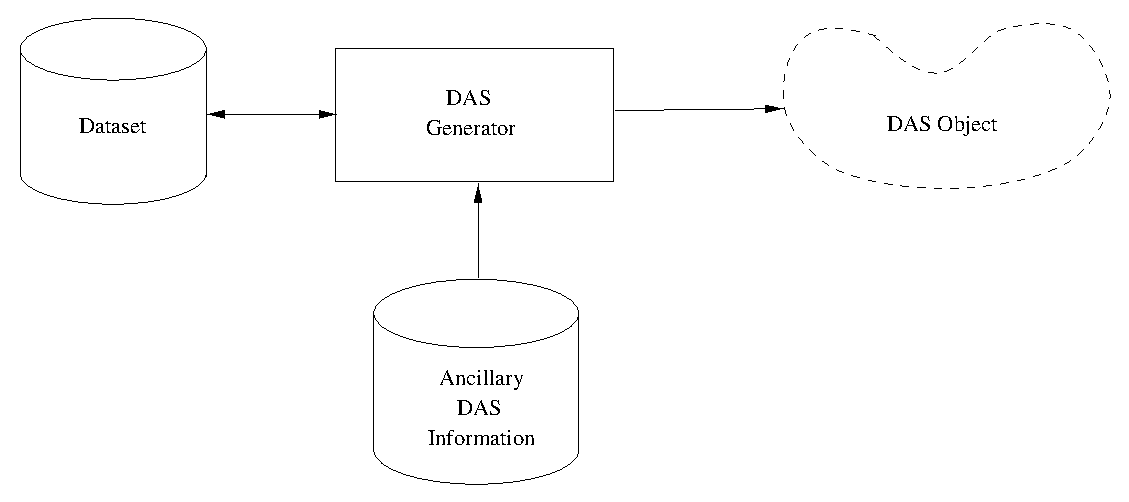
\epsfig{file=ancillary_das.eps,width=5.25in}
\caption{Information from the dataset along with and ancillary DAS object are
  combined into a single DAS object.}
\label{fig:ancillary}
\end{figure}

Clients will use this information by requesting it. It will be up to the
client to know to look for standard names, substitute the real name of the
variable for the standard name, etc. In the future we can make the system
more automatic. See the DODS User's Guide for more information about DAS
objects, attributes and ancillary attributes.

Figures~\ref{dspdds}~and~\ref{dspdas} show information for one of the image
files in the DSP image archive at GSO. The DAS shown (Figure~\ref{dspdas}) is
the \emph{ancillary} DAS file. In other words that is the information were
adding to the DAS so that when a client requests the DAS of one of the images
it will see the information shown there \emph{in addition to} the information
that the DSP server extracts from the file.

\begin{figure}
\begin{code}{c}
[dcz:/usr/local/DODS/src/dap-2.17] geturl -d $dsp
Dataset {
    Grid {
     ARRAY:
        Byte dsp_band_1[lat = 1024][lon = 1024];
     MAPS:
        Float64 lat[lat = 1024];
        Float64 lon[lon = 1024];
    } dsp_band_1;
    Float64 lat[lat = 1024];
    Float64 lon[lon = 1024];
} h97197120242;
\end{code}
\caption{DDS of a DSP Image file.}
\label{dspdds}
\end{figure}

\begin{figure}
\begin{code}{c}
[dcz:/usr/local/DODS/src/dap-2.17] geturl -a $dsp
Attributes {
    DODS_GLOBAL {
        String DODS_Interfaces "";   # No interfaces supported
        Int32 DODS_Standards 2;      # Class of this dataset/server
    }
    lat {
        String DODS_Name "Latitude"; # New information
        Alias DODS_Units units;      # Alias to existing attribute
        DODS_Parameter "...";        # Whatever the GCMD param. name is.
        DODS_Extent {
            Float64 DODS_Min_Max 34.7, 62.5;
        }
    }
    .
    .
    .
    dsp_band_1 {
        String DODS_Name "Sea Surface Temperature";
        String DODS_Units "counts";
        DODS_Parameter "...";        # Whatever the GCMD param. name is.
        DODS_Extent {
            Float64 DODS_Min_Max 0, 255;
            # Vertices of containing polygon (a box in this case)
            Float64 DODS_Containment 34.7, -70.0, 34.7, -50.0,
                                     62.5, -70.0, 62.5, -50.0;
        }
        DODS_Mapping_0 {
            String DODS_Unit "degC";
            Int32 DODS_Null 0, 1, 2, 3;
            Float64 DODS_Coefs 0.125, 2.5;
        }
    }
}
\end{code}

\caption{Possible entries into an ancillary DAS for the DSP Image in
  Figure~\ref{dspdds}. Parts of the DAS have been removed to make it more
  readable.} 

\label{dspdas}
\end{figure}

A more complicated situation is presented by
Figures~\ref{jpldds}~and~\ref{jpldas}. These figures show the DDS and an
ancillary DAS for the JPL Pathfinder file server discussed in
Section~\ref{sec:fileserver}. The server supports the date and time interfaces
which includes (unless we decide to change them) two functions which return a
standardized date and/or time value. Effectively those interfaces synthesize
a variable. How do we represent that synthesized variable in the ancillary
DAS? One way (shown) is to add a new attribute container for the variable and
include various `standard' names for it ({\tt DODS\_Min}, {\tt DODS\_Max},
\ldots).

\begin{figure}
\begin{code}{c}
[dcz:] geturl -d $jpl
Dataset {
    Sequence {
        String year;
        Sequence {
            String day;
            String hours;
            String minutes;
            String seconds;
            String DODS_URL;
        } Level_1;
    } Level_0;
} pathfinder;
\end{code}
\caption{DDS for the JPL Pathfinder File server}
\label{jpldds}
\end{figure}

\begin{figure}
\begin{code}{c}
[dcz:] geturl -a $jpl
Attributes {
    DODS_Global {
        # This server supports the date and time interfaces.
        String DODS_Interfaces "date", "time";
    }
    DODS_Time {
    .
    .
    .
    }
    .
    .
    .
    DODS_URL {
    }
}
\end{code}
\caption{Ancillary DAS for the JPL Pathfinder File Server. How do we include
  information about date/time?}
\label{jpldas}
\end{figure}

\subsection{Discovering a server's class}
\label{sec:classes}

There is a need to support multiple classes\footnote{Note to be confused with
  classes in OOP; really, `levels' would be a better word, but that is
  loaded with obscure meanings in the science data systems world.} of
datasets within DODS. One class of server provides the lowest level of
services. They return, via the DAS, DDS and Data objects, exactly what was
encoded with the data. In the case of some APIs (e.g., NetCDF) that
\emph{may} be a lot information while in the case of others (e.g., Matlab) it
will be next to nothing.  At the other end of the spectrum will be servers
which had extensive amounts of additional information about the dataset. We
should not plan on accessing this information using a functional interface
because, by default, DODS servers have \emph{no} functions. They are added on
a per server basis. However, the DAS object was specifically designed to hold
additional information about the dataset and its variables \emph{and} to be
extensible (without changing the underlying data).

Clients wanting information about a dataset's/server's class can examine the
attribute container {\tt DODS\_GLOBAL} for the attribute {\tt
  DODS\_Interfaces}. If present, it will give the class of the
server/dataset.  If absent, the client should assume the server/dataset is
class 0 (the lowest level of a dataset/server). See
Appendix~\ref{app:standard}.

\subsection{Discovering a server's interfaces}
\label{sec:interfaces}

To provide a way for clients to learn about various interfaces available from
a given server, we can describe those interfaces in an attribute called
{\tt DODS\_Interfaces}. Each interface will have a standard set of
functions which will be listed in an appendix of this paper. For example, one
interface previously described is the date/time interface. The
DODS\_interfaces attribute would only need to name the interface, not list
all of its functions, etc. It will be up to the clients to know which
interfaces do what. See Appendix~\ref{app:standard}.

\section{Using Scientific Units for Queries}

Users should be able to ask for data using Earth-science units. In the
current incarnation of DODS, if a user wants to read information from an
array or grid they must either read the entire data object or use array
indices to constrain the object. This is often hard to do since the mapping
between indices and Earth units can be complex. DODS needs to provide a
simple way for users to frame queries using the units in which the variables
are registered.



\section{Going Further}

Here are features which should be added to the base-line catalog services
described in this paper:

\begin{itemize}
  
\item Extend the catalog server so that it can use attributes of subordinate
  datasets as variables in its own dataset.  For example, suppose that a
  catalog for the AVHRR dataset lists Date, Time and URL. Each file in the
  dataset is referenced by one URL and the Date and Time columns of the
  catalog provide a way to choose a URL based on date and time. Now suppose
  that in each file (which is also a dataset) there is a variable called
  `lon' with DODS:Minimum and DODS:Maximum attributes. The `lon' variable
  from the files could be promoted to the catalog and, in the catalog, it
  would assume the values given by the Minimum and Maximum attributes.
  
  In order to promote an attribute up from a dataset to a catalog for that
  dataset, the attribute must be marked as \emph{promotable}. For a
  multi-file dataset, an attribute is promotable if it is preset and has the
  same value in all files. All attributes in single file datasets are
  promotable.
  
  Attributes promoted would be the DODS standard ones. The DODS:Name
  attribute of a dataset would be used to name the variable in the catalog.

\item Add an additional service that can hold an object, or reference to an
  object, without returning it. This service would allow clients to ask
  questions about the referenced object \emph{before} retrieving it.

\item Extend the catalog so that it can dereference URLs automatically and
  return complex objects.

\end{itemize}

\clearpage

\appendix

\section{Standard Attributes}
\label{app:standard}

These attributes must/should be present for a class 1 or 2 dataset. Next to
each attribute name is the lowest class of server that is required to have
that standard name in the DAS object. A class 2 server must have both class 1
and 2 attributes, while a class 1 server needed only the class 1 attributes.
A server that supplies none of these attributes is a class 0 server.

\begin{description}

\item [DODS\_GLOBAL: 1] This is an attribute container that holds other
  standard attributes which apply to the entire dataset and server.

  \begin{description}

  \item [Interfaces: 1] This attribute contains a vector of strings, each
    element of which names a standard interface supported by this server.
  \item [Standards: 1] An integer describes the class of this server
    and dataset. 0 $==$ some class 1 attributes missing, 1 $==$ no class 1
    attributes missing, some or all class 2 attributes missing, 3
    \ldots\footnote{Yes, there is a bit of a catch 22 here. If this attribute
      is missing then the client is on its own.}

  \end{description}

\item [DODS\_Time: 1] This attribute container holds information used by the
  DODS\_Time interface. These attributes provide a simple way to configure
  the DODS\_Time interface so that time data may be read from datasets
  without data providers writing C++ code. The information contained here will
  be expanded to cover a broader range of storage formats as dictated by
  demand. 
  
  \begin{description}
    
  \item [hours\_variable: 1] This holds the name of the variable in the
      dataset which contains hours information. If the variable is part of a
      Sequence, then it is assumed that that for each instance of the
      Sequence, the named variable contains hours information for that
      instance. The same applies to the following two attributes. 

    \item [minutes\_variable: 1] This holds the name of the variable which
      contains minutes information.

    \item [seconds\_variable: 1] This holds the name of the variable
      which contains seconds information.
      
    \item [gmt\_time: 1] This holds either the string `true' or `false'
      depending on whether the dataset's times are GMT/UTC times or not.

    \end{description}

\item [DODS\_Date: 1] This attribute container holds information used by the
  DODS\_Date interface that used in a way analogous to that held by the
  DODS\_Time attribute container.

  \begin{description}
    
    \item [year\_variable: 1] The name of the variable which contains the
      year information for a date. If this variable is part of a sequence,
      then it is assumed that it contains the year information for that
      sequence element.
      
    \item [year\_base: 1] If present, this Int32 attributes contains the base
      year for dates. For example, if a dataset stores the year 1998 as 98,
      year\_base would be 1900. If this is not present DODS will assume that
      a year 98 refers to 98 A.D.\footnote{This will almost certainly be
        wrong, but it is also better in the long run since `base 1900' dates
        are a bad idea.}

    \item [month\_variable: 1] The name of the variable which contains
      information about the month.

    \item [day\_variable: 1] The name of the variables which contains
      information about the month. If this attribute is used the
      \emph{year\_day\_variable} attribute should not be present. The results
      of defining both \emph{day\_variable} and \emph{year\_day\_variable}
      are undefined.

    \item [year\_day\_variable: 1] The name of the variable which contains
      year-day date information. For example, some datasets store year
      information in one variable and a day offset within the year in
      another. See \emph{day\_variable} for warnings about defining both that
      attribute and this one.

    \end{description}

\begin{quote}
  The DODS\_Date\_Time interface provides a way to compute with combined date
  and time values. The interface uses the DODS\_Date and DODS\_Time
  attributes. That is, the DODS\_Date\_Time\_Factory class will read from the
  DODS\_Date and DODS\_Time attributes. See Appendix~\ref{app:datetime} for
  more information about date and times in constraint expressions.
\end{quote}

\item [Variable name: 0] For each variable in a dataset, there is one attribute
  container with that variable's name. This is not part of the standard---
  there is always an attribute container for each variable name. The
  attributes listed below are \emph{per variable} attributes. They appear in
  each variable's attribute container.

  \begin{description}

  \item [DODS\_Name: 1] The name of this variable. We will need to build a
    dictionary of blessed names. Examples include \emph{Latitude}, \ldots
  \item [DODS\_Parameter: 2] The GCMD classification of this variable.
  \item [DODS\_Unit: 2] In what units are the variable's values.

  \item [DODS\_Extent: 2] This container attribute 
    \begin{description}
    \item [DODS\_Min\_Max: 2] A two element vector which contains the minimum
      and maximum values for this variable. Present only for scalars.
    \item [DODS\_Enum: 2] An enumeration of possible values for this variable.
      Present only for scalars. DODS\_Min/DODS\_Max and DODS\_Enum are mutually
      exclusive attributes
    \item [DODS\_Containment: 2] A vector of vertices of a polygon enclosing
      the data. The vector stores latitude/longitude information in the
      vector as $lat_{0},lon_{0}, \cdots, lat_{n},lon_{n}$.\footnote{Should
  this be made more general so as to include other types of containment?}
    \end{description}

  \item [DODS\_Mapping\_\emph{name}: 3] Provides information on mapping the
    values of this variable from DODS\_Unit to some other unit system. There
    can be more that more that one set of mapping attributes if there are more
    than one set of values.

    \begin{description}

    \item [DODS\_Coefs: 3] A vector containing $a_{0}, a_{1}, \cdots, a_{n}$
      where those values can be used in $y = a_{n}x^{n} + \cdots + a_{1}x +
      a_{0}$ to map values of the variable $x$ into new values $y$.
    \item [DODS\_Unit: 3] The Units of $y$ in the above are given by this
      attribute. 
    \item [DODS\_Null: 3] If any values of the variable are used to denote
      null or missing values they should be given here. If more than one
      value is used to indicate missing data, this attribute should be a
      vector of those values.

    \end{description}

  \end{description}

\end{description}

\section{Date/Time}
\label{app:datetime}

The date/time interface provides a standard way to query a dataset about
time-dependent information. The interface provides a set of functions which
can be used to select data using date and/or time and to retrieve date and/or
time information in a standard way. In addition to the functions, the
interface defines a standard representation for dates and times. These
representations are used by the functions and the return values. The intent
of this interface is to present a standardized \emph{view} of a dataset's
contents, not to standardize the data values themselves. Thus the functions
must be customized to a particular dataset; they must know how to read
date/time information using the local conventions of the dataset as well as
transforming the standard representations into the local ones for comparison.

\subsection{Representation of dates and times}

Dates will be represented as a string formated in one of two ways: either
using a year, month, day format or using a year and day-number format. See
Table~\ref{tab:dates}. Time will be represented as a string using hours,
minutes and seconds.\marginpar{\em \tiny How should we handle smaller
  times?} See Table~\ref{tab:times}. Combined date and time values will use a
colon to separate the two parts of the string (e.g., $<date>:<time>$).

Examples dates, times and date-time strings:

\begin{itemize}

\item 1 January 1998: {\tt 1998/1/1}
\item 4 February 982: {\tt 982/2/4}
\item 4:57pm: {\tt 16:57:00}
\item 1:23:45am: {\tt 1:23:45}
\item 1 January 1998 at 4:57pm: {\tt 1998/1/1:16:57:00}

\end{itemize}

\begin{table}
\caption{Grammar for dates}
\label{tab:dates}

\begin{center}
\begin{tabular}{|l|l|}
\hline
$<date>$       & $<year>/<month>/<day>$ \\
               & $ | <year>/<day-number>$ \\ \hline
$<year>$       & $0 \cdots 9999$ \\ \hline
$<month>$      & $1 \cdots 12$ \\ \hline
$<day>$        & $1 \cdots 31$ \\ \hline
$<day-number>$ & $1 \cdots 366$ \\ \hline
\end{tabular}
\end{center}

\end{table}

\begin{table}
\caption{Grammar for times}
\label{tab:times}

\begin{center}
\begin{tabular}{|l|l|}
\hline
$<time>$       & $<hours>:<minutes>:<seconds>$ \\ \hline
$<hours>$      & $0 \cdots 23$ \\ \hline
$<minutes>$    & $0 \cdots 59$ \\ \hline
$<seconds>$    & $0 \cdots 59$ \\ \hline
\end{tabular}
\end{center}

\end{table}

\subsection{Functions for projection and selection}

Three functions are defined for selection by date and/or time. Arguments
enclosed in [] are optional.

\begin{description}
  
\item [date($arg_{0}$, {[}$arg_{1}${]})] Return true for all values whose
  dates equal or fall between $arg_{0}$ or $arg_{0}$ and $arg_{1}$. In the
  later case the range is inclusive.
  
\item [time($arg_{0}$, {[}$arg_{1}${]})] Return true for all values whose
  times equal or fall between $arg_{0}$ or $arg_{0}$ and $arg_{1}$. In the
  later case the range is inclusive.
  
\item [date\_time($arg_{0}$, {[}$arg_{1}${]})] Return true for all values
  whose date-times equal or fall between $arg_{0}$ or $arg_{0}$ and
  $arg_{1}$. In the later case the range is inclusive.

\end{description}

Matching these selection functions are three projection functions. These are
used in the projection part of a constraint expression to ask for date/time
information as a variable in the values returned as a result of the
query.\marginpar{\em \tiny There are two schemes described earlier in
  this paper---this is one of them.}

\begin{description}
  
\item [DODS\_Date({[}$container${]})] Add the variable {\tt DODS\_Date} to
  the set of variables returned as a result of this query.  If $container$ is
  given, add {\tt DODS\_Date} not at the top-level of the DDS but to the
  named container.
  
\item [DODS\_Time({[}$container${]})] Add the variable {\tt DODS\_Time} to
  the set of variables returned as a result of this query. If $container$ is
  given, add {\tt DODS\_Time} not at the top-level of the DDS but to the
  named container.
  
\item [DODS\_Date\_time({[}$container${]})] Add the variable {\tt
    DODS\_Date\_Time} to the set of variables returned as a result of this
  query. If $container$ is given, add {\tt DODS\_Date\_Time} not at the
  top-level of the DDS but to the named container.

\end{description}

\subsection{Customizing the Date/Time interfaces for a particular dataset}

There are three ways to customize the Date/Time interfaces for a particular
dataset. Different customization options are provided since there is a wide
variety of storage forms and formats. The simplest option can be done without
any software development at all (see Section~\ref{custopt1}) while others
require that \Cpp\ software be written (See
Sections~\ref{custopt2}~and~\ref{custopt3}) .

\subsubsection{Using attributes to customize the Date/Time interfaces}
\label{custopt1}

If a dataset stores year, month, day or year and year-day information in
integer variables, then the Date interface may be set up using attributes.
See Section~\ref{app:standard} for information. Similarly, the Time and
Date\_Time interfaces may also be configured using attributes for datasets
which have the required information in Integer variables.

\subsubsection{Writing new factory classes}
\label{custopt2}

The attributes described in Section~\ref{app:standard} are read by
\emph{factory}\footnote{I'm using the term as it appears in the Java
  programming language documentation.} classes which configure themselves to
read the appropriate type object from the dataset (e.g., See the source files
{\tt DODS\_Date\_Factory.h} and {\tt DODS\_Date\_Factory.cc}). For each class
which implements one of the standard interfaces (DODS\_Time, DODS\_Date and
DODS\_Date\_Time) there is a matching factory class (DODS\_Date\_Factory,
\ldots).

For any dataset which does not store information in a way anticipated by the
current set of factory classes, users may modify or extend those classes or
replace one or more with new factory classes.

\subsubsection{Writing new interfaces}
\label{custopt3}

For some datasets the concept of a factory object which reads values may not
be appropriate. In this case, a new interface class may be written. In this
case the new class must be meshed with the constraint expression evaluator.
To do this three new functions (not member functions) must be written. The
source file {\tt ce\_functions.cc} contains examples of these three functions. 

In order to enable the CE evaluator to compare values using a standard
representation, you must register a comparison function. in the source file
{\tt ce\_function.cc}, look at the definition of {\tt bool func\_date(\ldots)}
for an example.  To enable the return of values using your new standard
interface class, you must define two new functions; one to run during the
evaluation of the projection part of the CE and one that is run during the
evaluation of the selection part of the CE. Look at the definitions of
{\tt void proj\_dods\_date(\ldots)} and {\tt bool sel\_dods\_date(\ldots)} in
{\tt ce\_functions.cc}, respectively, for examples for these. Note that the
{\tt bool func\_date(\ldots)} and {\tt void proj\_dods\_date(\ldots)} functions
must be registered with the DDS using {\tt add\_function(\ldots)}. To see an
example of this, look at {\tt ff\_dods.cc}.

%
% mail message explaining the odd interface

I think I've figured out where the problems lie with the decimal date
functions. If that is correct, I know how to fix the problems without too
much work. My explanation of the problem is long, sorry. Down at the bottom
is my proposed solution.

The problem:

In the file ce_functions.cc I define the `glue routines' that link the
DODS_Date, etc. classes to the functions called by the expression evaluator.
There are three types of functions: The comparison functions like

    bool func_date(int argc, BaseType *argv[], DDS &dds);

and selection and projection functions like:

    bool sel_dods_jdate(int argc, BaseType *argv[], DDS &dds);

    void proj_dods_jdate(int argc, BaseType *argv[], DDS &dds);

The first type of function is registered with the expression parser/evaluator
using: 

    dds.add_function("date", func_date);

That's how the parser knows that the symbol `date' is OK and is a function.
When the interpreter sees that a function has been parsed (RValue objects,
which hold the values to be interpreted for each clause of the CE, have
special fields for functions) it uses the mapping set up in the DDS to match
the symbol `date' to the C++ function `func_date'. All CE functions take the
same three arguments: an argument count, a vector of BaseType *'s and a DDS
reference. 

In ce_functions.cc func_date is defined as:

    bool
    func_date(int argc, BaseType *argv[], DDS &dds)
    {
        return comparison<DODS_Date, DODS_Date_Factory>(argc, argv, dds);
    }

Where `comparison' is the following template function (I love how templates
make things soooo much easier to understand... not :-)).

    template<class T, class T_Factory>
    bool
    comparison(int argc, BaseType *argv[], DDS &dds)
    {
        if (argc < 1 || argc > 2)
            throw Error(malformed_expr,
                        "Wrong number of arguments to a constraint expression 
                         function.");

        T t1(argv[0]);
        T t2;
        if (argc == 2)
            t2.set(argv[1]);

        T current = get_instance<T, T_Factory>(dds);

        if (argc == 2)
            return (t1 <= current) && (t2 >= current);
        else
            return (t1 == current);
    }

This means that the date function will compare two (or three, depending on
how its called) DODS_Date objects. It won't ever get DODS_Decimal_Year
objects.

In order to get variables added (synthesized) to the DDS two functions
are required. The `projection function' and the `selection function'. The
projection function is bound to a name using the DDS::add_function method.

    dds.add_function("DODS_JDate", proj_dods_jdate);

One of these `projection functions' looks like:

    void
    proj_dods_jdate(int argc, BaseType *argv[], DDS &dds)
    {
        if (argc < 0 || argc > 1)
            throw Error(malformed_expr,
    "Wrong number of arguments to projection function.\n\
    Expected zero or one arguments.");

        new_string_variable("DODS_JDate", dds, (argc == 1) ? argv[0] : 0);

        // Add the selection function to the CE

        dds.append_clause(sel_dods_jdate, 0); // 0 == no BaseType args

    }

Aside from the error message it does two things: Creates a string variable
and adds it to the DDS (new_string_variable(...) is messy but it just adds
a variable with the given name). The second line adds the `selection function'
as a clause in the current CE. This means that the function will be evaluated
every time the CE is evaluated. The `election function' sel_dods_jdate looks
like:

    bool
    sel_dods_jdate(int argc, BaseType *argv[], DDS &dds)
    {
        if (argc != 0)
            throw Error(malformed_expr,
    "Wrong number of arguments to internal selection function.\n\
    Please report this error.");

        DODS_Date current = get_instance<DODS_Date, DODS_Date_Factory>(dds);

        // Stuff the yyyy/ddd string into DODS_JDate.
        Str *dods_jdate = (Str*)dds.var("DODS_JDate");
        // By calling DODS_Date::get with the token `yd' I'm explicitly asking
        // for the year/day (pseudo juilian) date format. 5/27/99 jhrg
        string s = current.get(yd).c_str();
        dods_jdate->val2buf(&s);

        return true;
    }

Note that it always returns true so it does not affect the outcome of the CE;
this function is run only for its side effect which is to use the class and
its factory to read the current instance through the get_instance template
function. The first argument of that template provides the return type for
get_instance and the second tells how to build up the first using information
in the DAS. I.E.: The factory class parameterizes the DAS information for the
object.

    Aside: template are one way to having a single function return a
    different type depending on calling context.

Anyway, this `selection function' calls DDS::var() to read the synthesized
variable and grabs a local pointer to the synth variable. Then it uses the
get() method of `current', which is an instance of DODS_Date in the example,
to get the information from `current'. The object `current' is the return of
get_instance<...>(...) and is the DODS_Date corresponding to the current
state of the dataset. Usually that means that some variables in a Sequence
object are read and from their values a new DODS_Date is created (although it
does not have to be that done that way). The string is then stuffed into the
synth variable. That's how the value gets into the synth variable. Since the
`selection function' was added by the projection function during the parse of
the CE, and since the projection part of the CE always comes first, this
selection function will always be run before the regular selection functions
like `date', so the values are sure to be there when those regular election
functions are run (or other operations are performed in the selection part of
the CE).

    Aside: One way to optimize the date comparison function would be for it
    to look in the DDS (which it gets as a parameter) for a DODS_Date
    variable, and if it is there, use that variable's value rather than run
    get_instance<...>(...) a second time. I put the call to get_instance in
    there so that date and its ilk would be self-contained.

The problem here is that the sel_dods_decimal and proj_dods_decimal functions
have not been written and were not registered with the DDS. This means that
when the CE parser sees `DODS_Decimal' in the projection part of the CE, its
not going to know what to do. That symbol might still parse, but that is a bug
in parser; without a corresponding function it should generate a parse error.

The Solution: (sorry this is going on so long)

We can modify the DODS_Date_Time class to recognize <int>.<int> as a
fractional data/time value and initialize itself correctly. We can do this by
searching for the `.' and switching on that in the set member function. Then
we can overload the get() method so that it takes a token `dec' and, when
given that, returns a decimal date/time. That's how DODS_Date knows to return
y/m/d or y/d dates. In fact, we might want to extend both DODS_Date_Time and
DODS_Date.

Then we should write the proj_ and sel_ functions for the DODS_Decimal synth
variables. These would create either DODS_Date or DODS_Date_Time objects that
return their value as a string that looks like `<int>.<int>'. That's the
difference between DODS_Date and DODS_JDate; they are really the same class
but the sel_ functions for the synth variables use different forms of the
DODS_Date::get(...) member function.

The choice is between DODS_Date and DODS_Date_Time; I guess we have to use
the later. That means that comparisons will have to be done with the
date_time comparison function and not with date.

\end{document}    
